\documentclass[11pt,a4paper]{report}

% Language setting
% Replace `english' with e.g. `spanish' to change the document language
\usepackage[portuges]{babel}

% Set page size and margins
% Replace `letterpaper' with `a4paper' for UK/EU standard size
\usepackage[utf8]{inputenc}
\usepackage{graphicx}
\usepackage{url}
\usepackage{enumerate}
\usepackage{color}
\usepackage{multirow}
\usepackage{array}
\usepackage[pdftex]{hyperref}
\usepackage{listings}
\usepackage{enumitem}
\definecolor{codegreen}{rgb}{0,0.6,0}
\definecolor{codegray}{rgb}{0.5,0.5,0.5}
\definecolor{codepurple}{rgb}{0.58,0,0.82}
\definecolor{backcolour}{rgb}{0.95,0.95,0.92}

\lstdefinestyle{mystyle}{
    backgroundcolor=\color{backcolour},   
    commentstyle=\color{magenta},
    keywordstyle=\color{codegreen},
    numberstyle=\tiny\color{codegray},
    stringstyle=\color{codepurple},
    basicstyle=\ttfamily\footnotesize,
    breakatwhitespace=false,         
    breaklines=true,                 
    keepspaces=true,                 
    numbers=left,                    
    numbersep=2pt,                  
    showspaces=false,                
    showstringspaces=false,
    showtabs=true
}

\lstset{style=mystyle}

\title{PLC - Trabalho Prático 1\\
	\large Grupo nº5}

\author{Simão Pedro Batista Caridade Quintela \\ (A97444) 
        \and David José de Sousa Machado \\ (A91665)
        \and Hugo Filipe de Sá Rocha \\ (A96463)
       } %autores do documento
       
\date{\today} %data

\begin{document}

	\begin{minipage}{0.9\linewidth}
        \centering
		
\includegraphics[width=0.4\textwidth]{um.jpg}\par\vspace{1 cm}
		\href{https://www.uminho.pt/PT}
		{\scshape\LARGE Universidade do Minho} \par
		\vspace{0.6cm}
		\href{https://lcc.di.uminho.pt}
		{\scshape\Large Licenciatura em Ciências da Computação} \par
		\maketitle
		
		
\includegraphics[width=0.3\linewidth]{simao.jpg}
	    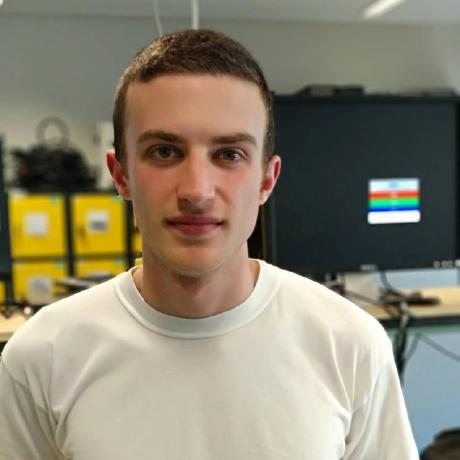
\includegraphics[width=0.3\linewidth]{david.jpg}	
        
\includegraphics[width=0.35\linewidth]{hugo.jpg}
        
		
	\end{minipage}
	
	\tableofcontents
	
	\pagebreak
	
	\chapter{Introdução}
% 
    \paragraph{}
    No âmbito da disciplina de Processamento de Linguagens e Compiladores foi-nos proposto pelo docente Pedro Rangel Henriques a realização de um trabalho prático com o objetivo de colocar em prática a utilização de expressões regulares para a análise de ficheiros de texto.

    \paragraph{}
    O trabalho prático consiste na resolução de, pelo menos, um problema em cinco propostos. Analisados os problemas acabamos por resolver o problema 1 (Processador de Pessoas listadas nos Róis de Confessados) e o problema 5 (Ficheiros CSV com listas e funções de agregação).

    \paragraph{}
    Neste documento estão apresentadas as soluções utilizadas para a resolução dos problemas abordados bem como a correspondente demonstração do funcionamento dos programas. 

    \chapter{Enunciados e Resoluções}
    \section{Processador de Pessoas listadas nos Róis de Confessados}
    \paragraph{}
    Construa agora um ou vários programas Python para processar o texto 'processos.txt' com o intuito de calcular frequências de alguns elementos (a ideia é utilizar arrays associativos para o efeito) conforme solicitado a seguir.

    \begin{enumerate}[label=\alph*)]
        \item Calcula a frequência de processos por ano (primeiro elemento da data);
        \item Calcula a frequência de nomes próprios (o primeiro em cada nome) e apelidos (o ultimo em cada nome) por séculos;
        \item Calcula a frequência dos vários tipos de relação: irmão, sobrinho, etc.
        \item Imprimir os 20 primeiros registos num novo ficheiro de output mas em formato JSON.
    \end{enumerate}

    \subsection{Resolução do problema}
    \paragraph{}
    Neste trabalho decidimos utilizar uma estratégia inicial semelhante em todas as alíneas que consiste em ler todas as linhas do ficheiro \textit{processos.txt} e guarda-las num array para depois poderem ser lidas na resolução das diferentes alíneas.

    \begin{enumerate}[label=\alph*.]
        \item Na resolução da alínea a. utilizamos um dicionário \textit{years} para guardar a frequência de processos por ano associando cada ano à frequência de processos. Para obtermos o ano e processo correspondente a cada linha do ficheiro utilizamos as funções \textbf{search} e \textbf{split}, e a seguinte expressão regular ([0-9]+)[:]{2}([0-9]{4}\-[0-9]{2}\-[0-9]{2}) \\
        \begin{lstlisting}[language=Python, caption=Alínea a]
def processFrequency():
    years = {}

    for line in lines:
        process_and_date = re.search('([0-9]+)[:]{2}([0-9]{4}\-[0-9]{2}\-[0-9]{2})', line)
    

        if process_and_date != None:
            process = process_and_date.group(1)
            date = process_and_date.group(2)
            data_splitted = re.split(r'-', date)
            year = data_splitted[0]

        
            if year not in years:
                years[year] = 1
            else:
                years[year] += 1

    return years
        \end{lstlisting}

        \item Na resolução da alínea b. utilizamos o dicionário \textit{centurys} que tem a seguinte estrutura:
        \begin{lstlisting}[language=Python]
# this is just an example:
centurys = {
    19: {
        "First": {"Candido": 10},
        "Last":  {"Faisca": 5}
    },
    20: {
        "First": {"Ivone": 130},
        "Last":  {"Costa": 2000}
    }
    
}
        \end{lstlisting}

        \paragraph{}
        Utilizamos a expressão regular \texttt{([0-9]{4})\-([0-9]{2})\-([0-9]{2})} com a função \textbf{search} para saber qual a data da linha lida.\\ Com a expressão regular \texttt{:([A-Za-z| ]+)(:)} e com a função \textbf{findall} conseguimos identificar o nome da pessoa processada, do pai e da mãe.\\Por fim, utilizando de novo a função \textbf{findall} e a expressão regular \texttt{([A-Z][A-Za-z ]+),([A-Za-z ]+). ?(?i:(Proc.[0-9]+))} conseguimos  identificar os nomes de pessoas que tiveram envolvidas noutros processos.

        \begin{lstlisting}[language=Python, caption=Alínea b]
def year_to_century(year):
    return -(-year // 100)

def nameFrequency():
    centurys = {}
    for line in lines:
        date = re.search(r'([0-9]{4})\-([0-9]{2})\-([0-9]{2})' ,line)
        names_in_dots = re.findall(':([A-Za-z| ]+)(:)', line)
        names_with_procs = re.findall('([A-Z][A-Za-z ]+),([A-Za-z ]+). ?(?i:(Proc.[0-9]+))', line)
 
        names = names_in_dots + names_with_procs
    
        if date:
            year = int(date.group(1))
            century = year_to_century(year)
            if century not in centurys:
                centurys[century] = {}
                centurys[century]["First"] = {}
                centurys[century]["Last"] = {}

        for name in names:
            person_name = name[0] 
            name_splitted = re.split(" ", person_name)
            first_name = name_splitted[0]
            last_name = name_splitted[-1]
            if first_name not in centurys[century]["First"]:
                centurys[century]["First"][first_name] = 1
            else:
                centurys[century]["First"][first_name] += 1

            if last_name not in centurys[century]["Last"]:
                centurys[century]["Last"][last_name] = 1
            else:
                centurys[century]["Last"][last_name] += 1
    return centurys
        \end{lstlisting}

        \item Na resolução da alínea c utilizamos um dicionário \textit{rel\_freq} para guardar a frequência de relações existente no ficheiro de texto. 
        
        Ao analisar o ficheiro reparamos que estes dois padrões que se repetiam:\\
        \begin{enumerate}
            \item \texttt{::Filho::Pai(opcional)::Mãe(Opcioal)::}\\
            \item \texttt{nome, relação parentesco, Proc.x} \\
        \end{enumerate}

        Para identificar o padrão \texttt{(a)} usamos a função \textbf{findall} e a expressão regular \texttt{:([A-Za-z| ]+):} . De notar que, no dicionário, o \textbf{Pai} e a \textbf{Mãe} são ambos contabilizados na entrada \textbf{Progenitor} visto que em várias linhas, por vezes a ordem pela qual aparece o nome dos mesmos é trocada. Para o efeito, e para não correr o risco de recolher informação errada optamos por coloca-los na mesma entrada. \\
        \\
        Para identificar o padrão \texttt{(b)}, utilizamos a função \textbf{findall} e a expressão regular \texttt{([A-Z][A-Za-z ]+),([A-Za-z ]+). ?(?i:(Proc.[0-9]+))} para identificar as restantes relações de parentesco com o processado.
    
        \begin{lstlisting}[language=Python, caption=Alínea c]
def relationFrequency():
    rel_freq = {}
    rel_freq["Progenitores"] = 0
    rel_freq["Filho"] = 0

    for line in lines:
        parents_and_son = re.findall(":([A-Za-z| ]+):", line)
    
        if parents_and_son:
            parents = parents_and_son[1:]
            rel_freq["Filho"] += 1
            rel_freq["Progenitores"] += len(parents)

        relations = re.findall("([A-Z][A-Za-z ]+),([A-Za-z ]+). ?(?i:(Proc.[0-9]+))", line)
        if relations:
            for relation in relations:
                if relation[1] not in rel_freq:
                    rel_freq[relation[1]] = 1
                else:
                    rel_freq[relation[1]] += 1

    return rel_freq
        \end{lstlisting}
    

    \item Para fechar o exercício 1 falta imprimir as primeiras 20 linhas do ficheiro \textit{processos.txt} em formato JSON.
    
    Para a resolução desta alínea utilizamos duas funções, uma para recolher informação, e outra para escrever informação no ficheiro JSON pretendido.

    A função \textbf{info\_to\_json} tem como objetivo recolher informação linha a linha (assegurando-se que não está a ler duas vezes a mesma linha), utilizando expresões regulares mostradas anteriormente, na seguinte forma:

        \begin{lstlisting}[language=Python, caption=Estrutura de dados alínea d]
# dada a seguinte linha tem-se
# 569::1867-05-23::Abel Alves Barroso::Antonio Alves Barroso::Maria Jose Alvares Barroso::Bento Alvares Barroso,Tio Paterno. Proc.32057.   Domingos Jose Alvares Barroso,Tio Materno. Proc.32235.::

    
json_info = { 
    575::1894-11-08 :{
        "Processo": "575",
        "Data": "1894-11-08",
        "Pessoa processada": "Abel Alves Barroso",
        "Pai": "Antonio Alves Barroso",
        "Mae": "Maria Jose Alvares Barroso",
        "Tio Paterno": "Bento Alvares Barroso",
        "Tio Materno": "Domingos Jose Alvares Barroso"
    }
        \end{lstlisting}

        \begin{lstlisting}[language=Python, caption=Função info\_to\_json]
def info_to_json():
    json_info = {}

    valid_lines = 0
    i = 0
    while valid_lines < 20:
        line = lines[i]

        if line != '':
            process_and_date = re.search('([0-9]+)[:]{2}([0-9]{4}\-[0-9]{2}\-[0-9]{2})', line)
            both = process_and_date.group(0)

            if both not in json_info:
                process = process_and_date.group(1)
                date = process_and_date.group(2)
            
            
                json_info[both] = {"Processo": process, "Data": date}

                son_and_parents = re.findall(':([A-Za-z| ]+)(:)', line)

                json_info[both]["Pessoa processada"] = son_and_parents[0][0]

                if len(son_and_parents) == 2:
                    json_info[both]["Mae"] = son_and_parents[1][0]
                else:
                    json_info[both]["Pai"] = son_and_parents[1][0]
                    json_info[both]["Mae"] = son_and_parents[2][0]

                relations = re.findall('([A-Z][A-Za-z ]+),([A-Za-z ]+). ?(?i:(Proc.[0-9]+))', line)
                if relations:
                    for relation in relations:
                        json_info[both][relation[1]] = relation[0]


                valid_lines+=1
    
        i+=1
    return json_info
        \end{lstlisting}

    \paragraph{}
    Posto isto, e tendo toda a informação necessária, basta utilizar a função definida por nós \textbf{write\_on\_json} para escrever toda a informação num ficheiro JSON.

    \begin{lstlisting}[language=Python, caption=Função info\_to\_json]
def write_on_json():
    json_info = info_to_json()    
    f = open('res.json', 'w')

    f.write('[\n')


    for (i,entry) in enumerate(json_info):
        f.write('   {\n')
        data = json_info[entry]
        for (j, key) in enumerate(data):
            f.write(f'       \"{key}\": \"{data[key]}\"')
            
            if j == len(data)-1:
                f.write('\n')
            else:
                f.write(',\n')
            

        if i == len(json_info)-1:
            f.write('   }\n')
        else:
            f.write('   },\n')

    f.write(']\n')
    f.close()
    \end{lstlisting}
    
    \end{enumerate}


    \chapter{Exemplos de funcionamento}
    \section{Processador de Pessoas listadas nos Róis de Confessados}
    \paragraph{}
    Nesta secção vamos mostrar o funcionamento do programa bem como a informação recolhida pelas funções previamente apresentadas.
    \subsection{Frequência de processos por ano}
    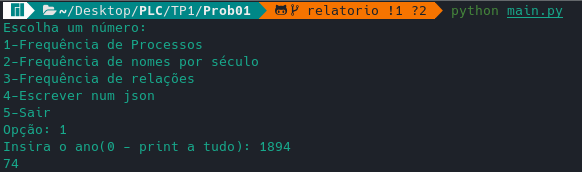
\includegraphics[width=0.8\linewidth]{alinea_a1.png} \\
	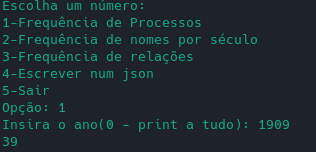
\includegraphics[width=0.8\linewidth]{alinea_a2.png}
    \paragraph{}
    Como podemos ver o programa está a fazer a contagem do número de processos por ano.
    
    \subsection{Frequência de nomes por século}
    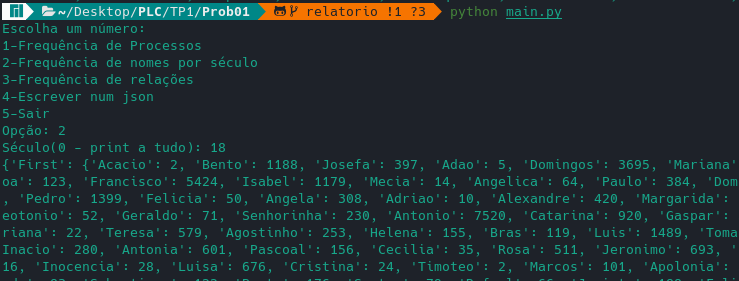
\includegraphics[width=0.8\linewidth]{alinea_b1.png} \\
	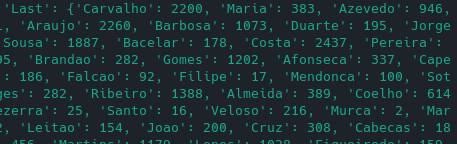
\includegraphics[width=0.8\linewidth]{alinea_b2.png}
    \paragraph{}
    Como podemos ver o programa está a fazer a contagem do número de nomes e apelidos por século.

    \subsection{Frequência de relações por século}
    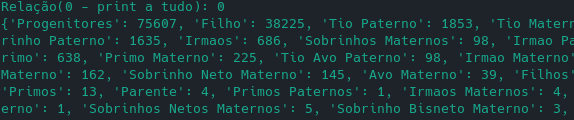
\includegraphics[width=0.8\linewidth]{alinea_c1.png} \\
    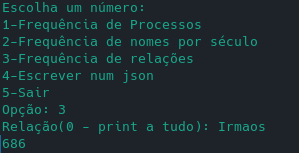
\includegraphics[width=0.8\linewidth]{alinea_c2.png}

    \paragraph{}
    Como podemos ver o programa está a fazer a contagem do número de relações.

    \subsection{Escrever as 20 primeiras linhas num JSON}
    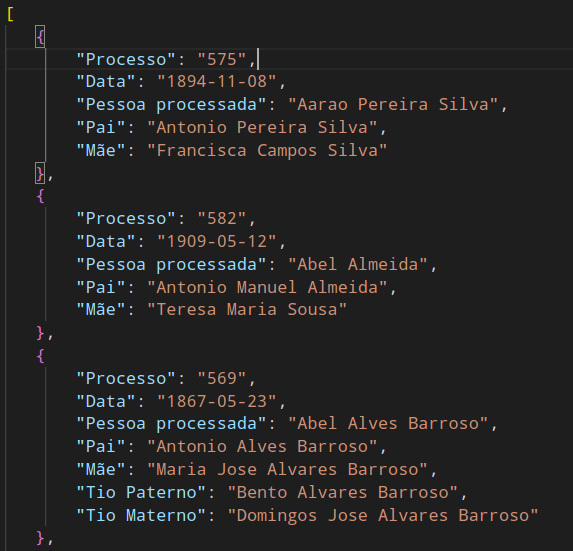
\includegraphics[width=0.8\linewidth]{alinea_d1.png} \\
    \paragraph{}
    Como podemos ver o programa está a escrever corretamente no ficheiro JSON.
    
\end{document}
